\section{Filtro de efecto de audio dentro del \textit{codec} de audio y configuración}



\begin{enumerate}
    \item  Antes de intentar hacer uso del  \textit{codec} se debe indagar sobre las características y forma de utilizar el método de filtrado que este dispositivo incluye. Para esto se recurre al \textit{datasheet} de la tarjeta la \href{https://www.ti.com/lit/ds/symlink/tlv320aic3106.pdf?ts=1628519638980&ref_url=https}{TLV320AIC3106}  provisto por Texas Instrument \footnote{Ver en \href{https://www.ti.com/lit/ds/symlink/tlv320aic3106.pdf?ts=1628519638980&ref_url=https}{https://www.ti.com/lit/ds/symlink/tlv320aic3106.pdf?ts=1628519638980&ref_url=https} }.
    
    En la sección \textbf{10.3.3.3.1 Digital Audio Processing for Playback} se describe la estructura del filtro y como programar el bloque asociado para poder utilizarlo en un proyecto. El filtro consta de dos filtros biquad en cascada, cuyos parámetros son modificables a conveniencia y se rigen por la siguiente ecuación 
    
    
    
    $$   H(z) = \left (\frac{N_0 + 2\cdot N_1 \cdot z^{-1} + N_2 \cdot z^{-2}}{ 32768 - 2\cdot D_1 \cdot z^{-1} - D_2 \cdot z^{-2}} \right ) \cdot   \left (\frac{N_3+ 2\cdot N_4 \cdot z^{-1} + N_5 \cdot z^{-2}}{ 32768 - 2\cdot D_4 \cdot z^{-1} - D_4 \cdot z^{-2}} \right ) $$
    
    
    Donde tal como se mencionó se tiene libertad para definir los parámetros \textit{N0-5} y \textit{D0-5} asociados a ambos filtros. Además se debe tener en cuenta el signo en los parámetros dado que la expresión que se ha usado a lo largo de este curso para el diseño e implementación de filtros biquad difiere con la descrita en el \textit{datasheet}
    
    $$ H(z) = \left (\frac{b_0 + 2\cdot b_1 \cdot z^{-1} + b_2 \cdot z^{-2}}{ 1 - 2\cdot a_1 \cdot z^{-1} - a_2 \cdot z^{-2}} \right )$$
    
    
    Otra sección relevante del \textit{datasheet}  es la \textbf{10.6 Register Maps} la que describe la forma en que se guardan los parámetros definidos en los registros de memoria del dispositivos, donde se indica que los parámetros se dividen  en dos registros, cada uno de 8 bits para poder abarcar el rango $[-32768, 32768]$
    
    Finalmente resulta útil conocer como modificar la amplitud de la salida generada por el dispositivo, esto se encontró en la sección \textbf{ 10.6.1 Output Stage Volume Controls} y será relevante para el proceso que se describirá a continuación.
    
    \item Se implementa en MATLAB un script que permite encontrar los coeficientes de los filtros biquad con el fin de obtener una respuesta suficientemente cercana a la respuesta en frecuencia deseada. Cabe destacar que por la limitante impuesta por el número de bits se debe corregir la amplitud  de uno de los filtros para poder trabajar dentro del rango de valores permitido, en este caso se corrige multiplicando por un factor de 0.8 veces.

\newpage    
    \begin{lstlisting}

%Coeficientes del filtro de orden 4
F = [0 221 1764 4410 6615 8820 22050]/22050;
%correccion para entrar en [-32768, 32768]
A_corr = [2.1 2 1.3 1 1 1.2 1.5]*0.8;


%obtencion de coeficientes
[b,a] = yulewalk(4,F,A_corr);

[h,w] = freqz(b,a);


%obtencion de coeficientes para los filtros
[sos, g] = tf2sos(b,a);

b1 = sos(1,1:3)
a1 = sos(1,4:6)

b2 = sos(2,1:3)
a2 = sos(2,4:6)

\end{lstlisting}


En la figura \ref{freqz} se pueden ver las gráficas obtenidas para la respuesta en frecuencia ideal y la respuesta en frecuencia generada con el script.

\begin{figure}[H]
    \centering
    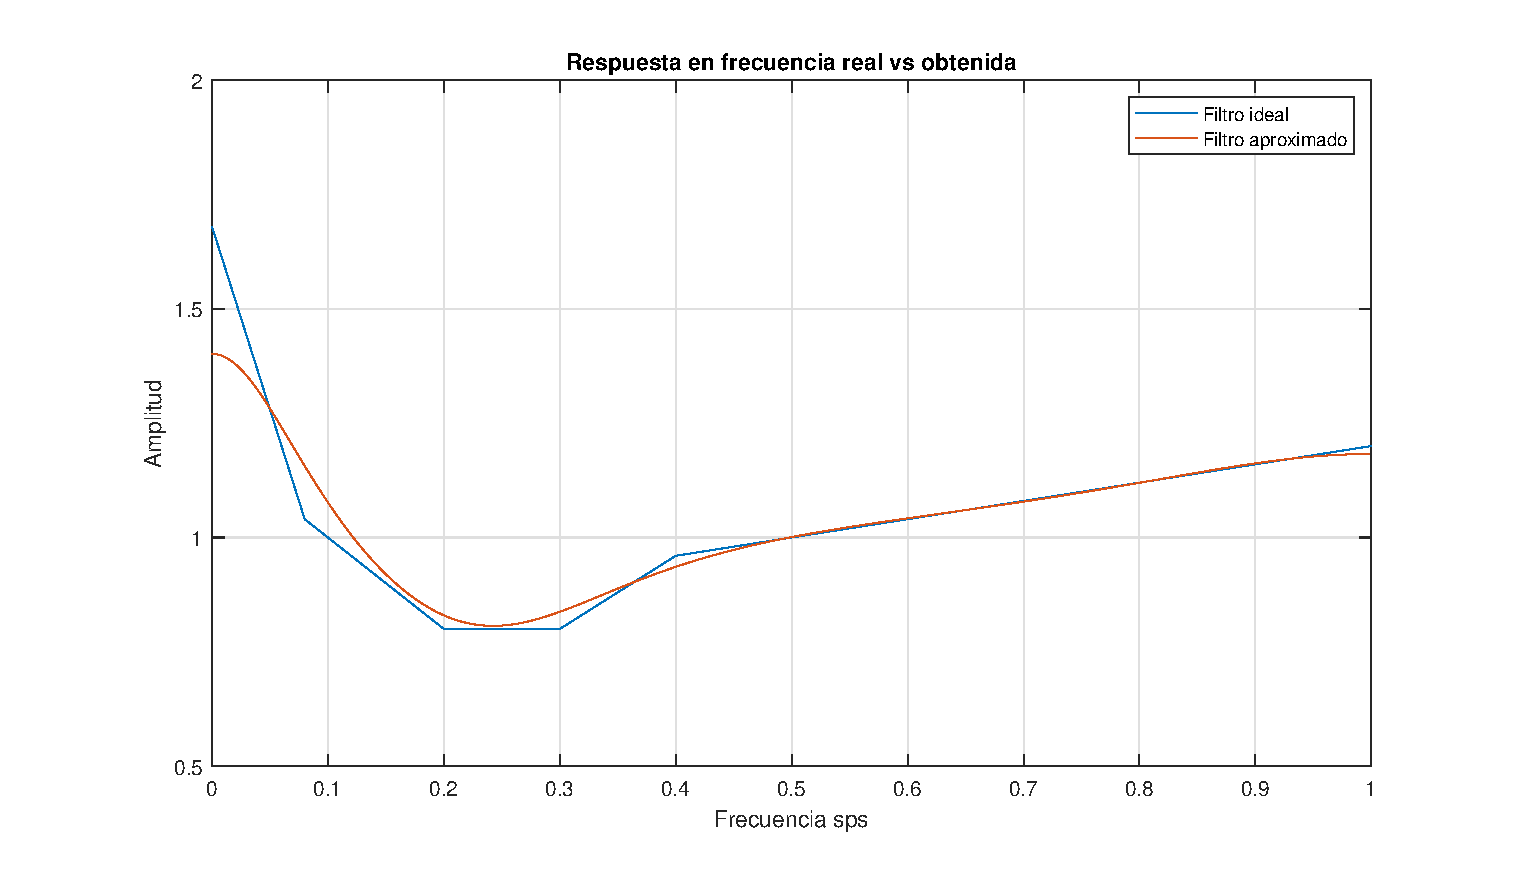
\includegraphics[scale = 0.6]{figures/freqz.eps}
    \caption{Respuestas en frecuencias ideal y obtenida mediante MATLAB}
    \label{freqz}
\end{figure}
    
Los coeficientes para los filtros biquad obtenidos mediante la función \textit{tf2sos} se muestran en la figura \ref{parámetros}

\begin{figure}[H]
    \centering
    \includegraphics[scale = 0.6]{figures/parametros.png}
    \caption{coeficientes obtenidos mediante \textit{tf2sos} para configurar los filtros biquad del \textit{codec} de audio.}
    \label{parámetros}
\end{figure}
    
    
Se debe considerar la discrepancia de signos que se señaló anteriormente para los coeficientes antes de utilizarlos como parámetro en el dispositivo. Además se debe recordar que para poder trabajar dentro del rango adecuado permitido por el dispositivo corrigió la ganancia  del filtro por un factor de 0.8, este efecto se debe corregir y se puede hacer corrigiendo el volumen de salida de audio del dispositivo (tal como se indica en la sección 10.6.1 Output Stage Volume Controls del \textit{datasheet})



\end{enumerate}